\documentclass[tikz]{standalone}
\usepackage{tikz}
\usetikzlibrary{arrows.meta,positioning,shapes.geometric,shapes.misc,fit,backgrounds,calc,decorations.pathreplacing}

\definecolor{cEmpirical}{HTML}{2B7A78}
\definecolor{cConjectured}{HTML}{C07C38}
\definecolor{cVerifier}{HTML}{A04050}

\begin{document}
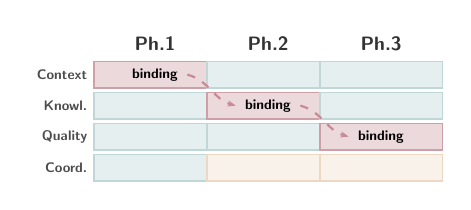
\begin{tikzpicture}[scale=0.82,
    cell/.style={minimum width=1.55cm, minimum height=0.34cm, font=\tiny\sffamily, inner sep=1pt},
    hi/.style={cell, fill=cVerifier!20, draw=cVerifier!50},
    lo/.style={cell, fill=cEmpirical!12, draw=cEmpirical!30},
    md/.style={cell, fill=cConjectured!10, draw=cConjectured!30},
    lbl/.style={font=\tiny\sffamily\bfseries, text=black!70, anchor=east},
    plbl/.style={font=\scriptsize\sffamily\bfseries, text=black!80}
]
\def\rh{0.48}
\def\cw{1.75}

\node[plbl] at (0, 0) {Ph.1};
\node[plbl] at (\cw, 0) {Ph.2};
\node[plbl] at (2*\cw, 0) {Ph.3};

\node[lbl] at (-0.9, -\rh) {Context};
\node[lbl] at (-0.9, -2*\rh) {Knowl.};
\node[lbl] at (-0.9, -3*\rh) {Quality};
\node[lbl] at (-0.9, -4*\rh) {Coord.};

\node[hi] at (0, -\rh) {\textbf{binding}};
\node[lo] at (0, -2*\rh) {};
\node[lo] at (0, -3*\rh) {};
\node[lo] at (0, -4*\rh) {};

\node[lo] at (\cw, -\rh) {};
\node[hi] at (\cw, -2*\rh) {\textbf{binding}};
\node[lo] at (\cw, -3*\rh) {};
\node[md] at (\cw, -4*\rh) {};

\node[lo] at (2*\cw, -\rh) {};
\node[lo] at (2*\cw, -2*\rh) {};
\node[hi] at (2*\cw, -3*\rh) {\textbf{binding}};
\node[md] at (2*\cw, -4*\rh) {};

\draw[-{Stealth[length=3pt]}, thick, cVerifier!60, dashed]
    (0.5, -\rh) to[out=-15, in=165] (\cw-0.5, -2*\rh);
\draw[-{Stealth[length=3pt]}, thick, cVerifier!60, dashed]
    (\cw+0.5, -2*\rh) to[out=-15, in=165] (2*\cw-0.5, -3*\rh);

\end{tikzpicture}
\end{document}
